\section{Problems}

\subsection{Statement of the Problems}

Many citizens find themselves under the pressure over moderate and too busy to
pursue for happiness. They are in unhealthy mental conditions but lack for
convenient ways to get happiness. People have tried to get happiness since the
happiness lesson in Havard, aiming to teach people to be happy, has become one
of the most popular courses. According to China Daily, many high school students
find themselves under high pressure, which is shown in the graph below. Even
though they want to do some exercise sometimes, the space is limited. 

\begin{figure}[H]
    \centering
    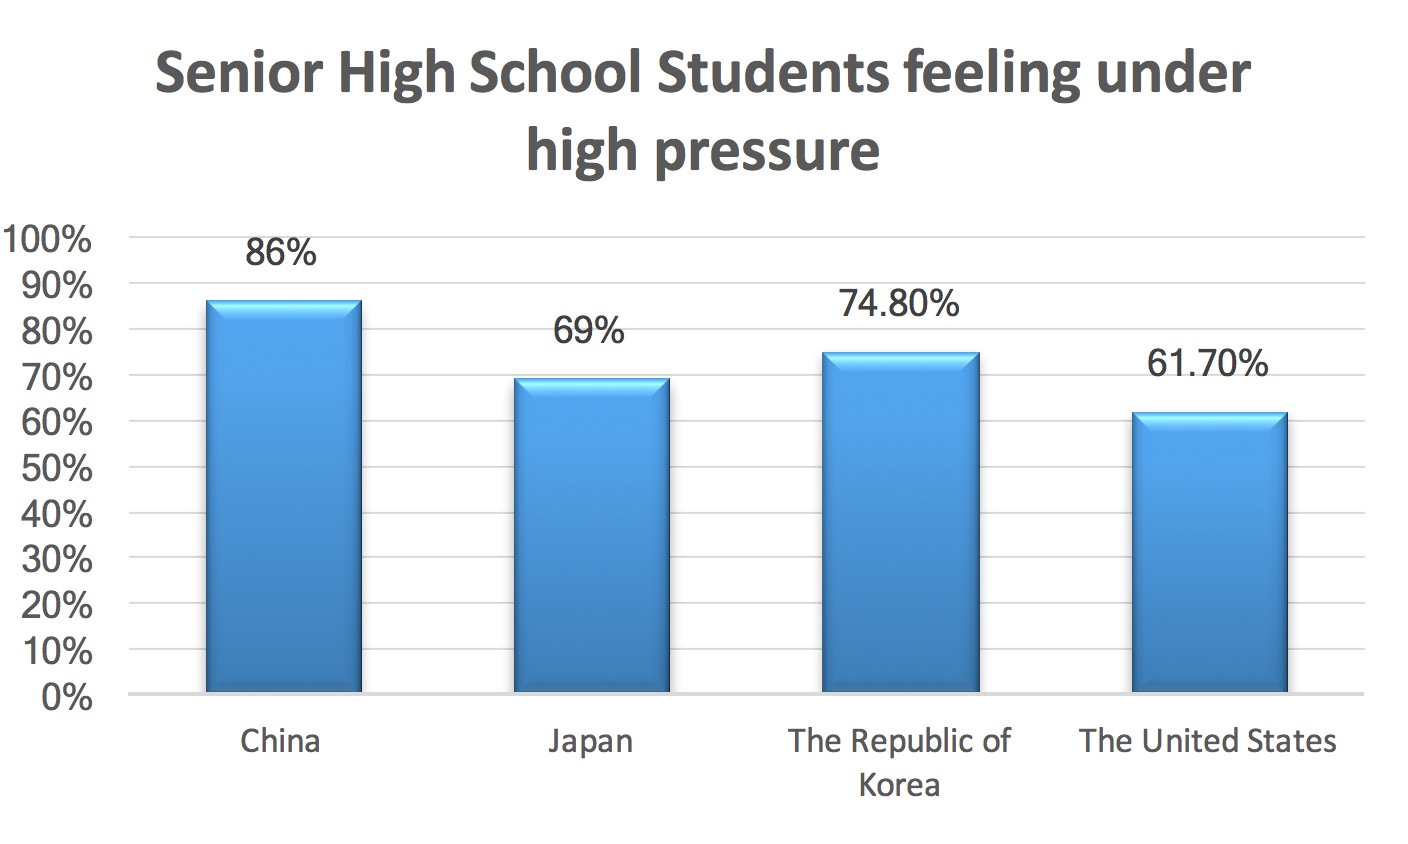
\includegraphics[width=13cm]{Pics/Problems1}
    \caption{Proportion of Senior High School Students under High Pressure}
\end{figure}

We choose dance to help people relax because it is convenient and low cost.
Compared to other healthy relaxing ways like jogging and walking, dancing can be
indoors, not influenced by the weather or the air pollution. The cost for dance
is quite low.  
Traditional dancing machines are not suitable enough for people who want to get
happiness from dancing. 

\begin{enumerate}[\hspace{2em} 1.]
    \item It does not meet home entertainment needs well because of large area
      occupation and high price. 
    \item It is unavailable for people with jobs and students in the work places
      or study rooms. 
    \item It stresses acrobatics , which is difficult for beginners. 
\end{enumerate}

As a result, traditional dancing machine cannot provide users with anytime and
anywhere dance. 

\subsection{Summary of Problems}

In summary, people need ways to relax because they are busy and under pressure.
Dance can help people to get happiness, but traditional dancing machine exists
these problems: 

\begin{enumerate}
    \item Large area occupation and high price
    \item Unavailable in most places
    \item Difficult for beginners
\end{enumerate}

